\documentclass[a4paper,13pt]{report}
\usepackage{polski}
\usepackage[utf8]{inputenc}
\usepackage[margin=1in,left=1.5in,includefoot]{geometry}
\usepackage{fancyhdr}
\usepackage{wrapfig}

\pagestyle{fancy}
\usepackage{graphicx}

\graphicspath{ {./images/} }

\begin{document}

\begin{titlepage}

\title{Praca inżynierska}
\author{Kamil Susek}
\date{September 2020}

\maketitle
\end{titlepage}
\chapter{Wprowadzenie}
\section{Temat projektu.}
Tematem pracy jest zaprojektowanie oraz implementacja uproszczonego systemu głosowania elektronicznego on-line. System powinien zostać opracowany od strony teoretycznej, a wybrane fragmenty powinny zostać zaimplementowane. Bezpieczeństwo systemu powinno zawierać elementy technologii Blockchain.
\section{Cele i założenia projektu.}
Realizację projektu można podzielić na dwie części. Pierwszą częścią jest zaprojektowanie od strony teoretycznej systemu elektronicznego głosowania on-line, na podstawie przeglądu istniejących rozwiązań. Za zabezpieczenie wyborów, przed fałszowaniem odpowiadać będzie technologia Blockchain. Realizacja drugiej części polega na implementacji wybranych fragmentów systemu.
Do wybranych fragmentów należą: 
\begin{itemize}
    \item aplikacja serwerowa, która zajmuje się obsługą Blockchain'u,
    \item aplikacja serwerowa, której zadaniem będzie obsługa zapytań do bazy danych całego systemu, 
    \item aplikacja kliencka, przeznaczona dla administratora wyborów, udostępnia możliwość kreatora wyborów,
    \item aplikacja kliencka, w formie aplikacji webowej, która pozwala na zalogowanie i  oddanie głosu.
\end{itemize}
\section{Wykorzystane technologie.}


\newpage
\chapter{Blockchain}
Technologia Blockchain to stosunkowo nowe rozwiązanie. Pierwsze zastwosowanie tej technologii miało miejsce w roku 2009, w popularnej kryptowalucie bitcoin. Zadaniem Blockchainu było księgowanie transakcji. Od tego czasu można zauważyć zwiększanie się zainteresowania tą technologią, co przekłada się na powstawanie nowych kryptowalut i nowych rozwiązań Blockchain (Blockachain 2.0, 3.0).
\section{Architektura Blockchain}
Blockchain to łańcuch bloków, które przechowują dane. Każdy blok przechowuje zabezpieczone kryptograficznie informacje, o poprzednim bloku i w ten sposób tworzy się trudny do modyfikacji łańcuch. Technologia Blockchain wykorzystuje rozproszoną sieć (Peer to Peer), w celu przechowywaniu kopii łańcucha w zdecentralizowanym systemie. Zdecentralizowane węzły komunikują się, w celu utrzymania spójności przechowywanych łańcuchów. Takie rozwiązanie pozwala zwiększyć bezpieczeństwo przechowywanych danych.
\subsection{Łańcuch bloków}
Łańcuch bloków w systemie Blockchain pełni funkcje struktury danych. Jego budowa przypomina trochę listę jednokierunkową, jednak zamiast wskaźników na poprzedni element, blok przechowuje hash poprzedniego elementu. Hash to wygenerowany za pomocą odpowiedniej funkcji kryptograficznej (funkcji skrótu) ciąg bajtów. Hashowanie jest operacją jednokierunkową, co oznacza brak możliwości odczytania danych wejściowych na podstawie wartości wygenerowanej przez hash.
Do popularnych funkcji skrótu należą SHA i MD5, jednakże należy pamiętać, że co jakiś czas te rozwiązania się zmieniają, ponieważ odkrywane są w nich luki.

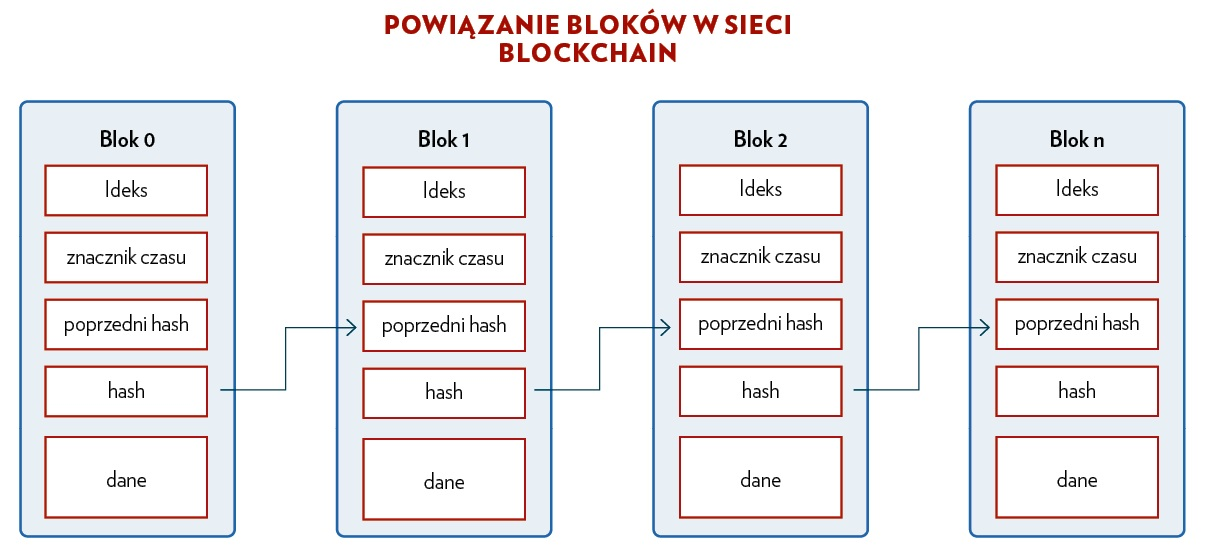
\includegraphics[width=\textwidth]{images/łańcuch_bloków.jpg}

Na łańcuchu bloków, jak na każdej strukturze danych można wykonywać operacje. W tym przypadku jednak operacje takie jak usuwanie bloku, lub jego modyfikacja nie mają sensu, ponieważ mechanizmy zastosowane w łańcuchu mają na celu zabezpieczenie przed modyfikacją danych w bloku. Najczęściej wykorzystuje się operacje dodawania bloku i sprawdzenia spójności łańcucha.

Dodanie bloku to dołączenie do tablicy bloków (bądź innej struktury łączącej lub indeksującej bloki) nowego bloku, w którym w pole "poprzedni hash" wpisywana jest wartość hash poprzedniego bloku. Następnie w świeżo dodanym bloku z wykorzystaniem funkcji skrótu liczymy hash z pól przechowujących dane, poprzedni hash i znacznik czasu.  

Sprawdzenie spójności łańcucha to przeliczenie hasha każdego bloku i porównanie go z polem "poprzedni hash" następnego bloku. Jest to główny mechanizm pozwalający wykryć niespójność w łańcuchu bloków, lecz nie należy tego mylić z problemem niespójności, w rozproszonym systemie Blockchain.

\subsection{Sieci Peer to Peer}

Ważną cechą Blockchainu, z punktu widzenia bezpieczeństwa jest wykorzystanie sieci P2P, w celu utworzenia rozproszonej sieci przechowującej dane. Tak zabezpieczone łańcuchy danych są jeszcze trudniejsze do podmiany, ponieważ trzeba podmienić każdą kopie znajdującą się w sieci.  

Sieć Peer to Peer to grupa urządzeń (węzłów), które komunikują się ze sobą w celu przechowywania i udostępniania wspólnych danych. Każde indywidualne urządzenie w sieci określane jest jako węzeł. Połączone ze sobą węzły tworzą rozproszoną sieć. Dodatkowo w przypadku, gdy żaden z węzłów nie wpływa w sposób znaczący na sieć, to można powiedzieć, że jest ona zdecentralizowana.

Za utrzymanie takiej sieci odpowiedzialność przejmują węzły, których zadaniem jest przechowywanie kopii danych i ich udostępnianie. Wykonywanie tych operacji jest przeprowadzane przez specjalne oprogramowanie, w które wyposażone są urządzenia tworzące węzły.

Takie sieci cechują się wysokim zabezpieczeniem przeciwko atakom cybernetycznym, ze względu na ilość węzłów w sieci, które przechowują kopie danych. Aby zniszczyć taką sieć należy zlokalizować i zaatakować wszystkie węzły.

Peer to Peer jest przykładem ciekawego zastosowania architektury klient-serwer. Architektura klient serwer polega na podzieleniu systemu na stronę kliencką, która zajmuje się wysłaniem żądań do serwera oraz na stronę serwerową, której zadaniem jest odpowiadanie na żądania, przechowywanie danych i operowanie na tych danych. W sieci P2P węzeł pełni role zarówno serwera, jak i klienta. Przykładowo węzeł może żądać przesłania danych od innego węzła, równocześnie odpowiadając na żądanie kolejnego węzła.
\subsection{Konsensus}
Węzły sieci Blockchain komunikują się ze sobą, w celu dystrybucji nowego bloku w sieci, oraz w celu osiągania konsensusu. Konsensus w sieci Blockchain to stan sieci, w którym zawartość łańcucha, w każdym węźle jest prawidłowa. Istnieje wiele metod osiągania konsensusu w sieciach Blockchain.

\subsubsection{Proof of work}

Proof of work to najczęściej wykorzystywany algorytm uzyskiwania konsensusu. Algorytm ten wykorzystywany jest podczas tworzenia nowego bloku. Nowy blok wysyłany jest do wszystkich węzłów w sieci, które w celu dodania bloku do swojego łańcucha muszą zostać zatwierdzone. Na tym etapie algorytmu mamy do czynienia z popularnymi "koparkami" Bitcoinów. Aby blok został zatwierdzony węzeł musi wykonać pracę, czyli dołożyć swoją moc obliczeniową. Moc obliczeniowa wykorzystywana jest do hashowania zestawu danych bloku, tak aby uzyskać określony wcześniej rezultat (np. hash musi się zaczynać od pięciu zer). Praca ta wykonywana jest przez węzeł i jest określana jako mining (ang. wydobywanie), jest to zadanie wykonywane przez wspomniane 
koparki, które za wykopanie bloku otrzymują specjalne środki w walucie Bitcoin. W typowych rozwiązaniach dla Bitocoinu poziom trudności dodania nowego bloku jest tak skonstruowany, aby nowe bloki były dodawane, w odstępach około 10 minutowych. 

Takie rozwiązanie premiuje węzły, o większej mocy obliczeniowej. Dlatego w celu utrzymania spójności danych należy przeprowadzać synchronizację węzłów. Synchronizacja przebiega nastepująco: 
każdy węzeł rozsyła do całej sieci swój łańcuch, węzły porównują długość swojego łańcucha z nadesłanym łańcuchem i w węźle zapisywany jest dłuższy łańcuch. 

Proof of work to rozwiązanie towarzyszące architekturze Blockchain, od momentu jej powstania, jednakże w miarę upływu czasu, wraz ze zwiększaniem się popularności Bitcoinów i zwiększaniem się mocy komputerów, powstały całe przedsiębiorstwa zajmujące się "kopaniem" Bitcoinów. Popularyzacja kopania Bitcoinów prowadzi do przejęcia tego rynku przez przedsiębiorstwa dysponujące całymi magazynami komputerów, które zajmowały się kopaniem Bitcoinów. Sam rozwój rynku nie jest  szkodliwy dla kryptowaluty, jedynie znacznie zmniejsza konkurencję rynku, eliminując pojedynczych kopaczy, którzy nie posiadają w domu pokoju wypełnionego "koparkami". 

Głównym problemem tego rozwiązania jest zużycie energii elektrycznej. Według badań naukowych z roku 2018, przeprowadzonych na Monachijskim Uniwersytecie Technicznym oraz Instytucie w Massachusetts (MIT), wydobywanie Bitcoina pochłonęło 45,8 TWh. Dla porównania w Polsce, w roku 2017 produkcja energii elektrycznej wyniosła 170,3 TWh. Aby pokazać skalę wzrostu wykorzystania energii elektrycznej przez Bitcoin, należy przytoczyć badania z roku 2019. Naukowcy z Uniwersytetu w Cambridge oszacowali, że światowe roczne zużycie energii elektrycznej przez Bitcoin jest równe 58,93 TWh. Dla porównania Szwajcaria zużywa rocznie 58,46 TWh. 

Należy również wziąć pod uwagę, że generowanie energii elektrycznej uwalnia do atmosfery szkodliwe substancje, których w obecnych czasach staramy się ograniczać. Głównym przeznaczeniem Bitcoinu jest bezpieczne księgowanie transakcji, jednak nie jest to jedyne rozwiązanie na rynku. Według wspomnianego już badania naukowców z Uniwersytetu w Cambridge, Bitcoin odpowiada za mniej niż 100 mln. operacji finansowych rocznie, natomiast tradycyjne systemu księgowania przeprowadzają około 500 mld. takich transakcji. W tym przypadku widać jak bardzo nieopłacalny jest algorytm Proof of Work, jednakże pomimo tego wciąż jest on najczęściej używany w rozwiązaniach Bitcoin.

W tym algorytmie czynnik wkładu fizycznych zasobów, jest głównym motywatorem do uczciwego postępowania. Nagroda otrzymywana jest tylko za prawidłowe zweryfikowanie bloku, dlatego węzeł próbujący obejść zabezpieczenia lub sfałszować zawartość bloku, w przypadku niepowodzenia traci zainwestowane zasoby.

Ogrom inwestowanych zasobów wpływa również na bezpieczeństwo sieci. Duża zdecentralizowana sieć Blockchain dysponuje ogromną mocą obliczeniową, na jej moc składa się moc wszystkich węzłów w sieci. Węzły różnią się mocą obliczeniową, natomiast decentralizacja sieci sprawia, że żaden z węzłów nie może przejąć kontroli nad całą siecią. Im większa decentralizacja tym bardziej zmniejsza się wpływ pojedynczego węzła na całą sieć. Co innego, gdy do sieci dołączona zostanie grupa węzłów, które będą stanowiły 51\% mocy obliczeniowej sieci oraz będą ze sobą współpracowały, działając na szkodę sieci. Taki scenariusz nazywany jest atakiem 51\%. 

W przypadku algorytmu Proof of Work atak 51\% jest bardzo rzadkim zjawiskiem, gdyż jest on bardzo drogi. Atak ten może być opłacalny jedynie wtedy, gdy atakujący chce zdestabilizować sieć. W przypadku Bitcoin'a destabilizacja sieci nie ma większego sensu, ponieważ dysponując taką mocą obliczeniową można uzyskać ogromne przychody z kopania Bitcoin'a, dodatkowo uzyskanie takiej mocy obliczeniowej w rozrastających się sieciach Blockchain dla Bitcoin'u jest na tyle drogie, że w teorii jest uznawane za nieosiągalne. Z tego powodu, w przypadku sieci Blockchain skupionych na przechowywaniu danych, bardzo ważne jest zadbanie o jak największe rozproszenie węzłów w sieci P2P i zwiększenie mocy obliczeniowej.

\subsubsection{Proof of Stake}

Proof of Stake to kolejny algorytm używany do osiągania konsensusu w sieciach Blockchain. Jego największe zalety, to rozwiązanie problemu zużywania ogromnych ilości zasobów energii elektrycznej przez algorytm Proof of Work.

Działanie algorytmu Proof of Stake polega na wybieraniu spośród dostępnych węzłów sieci Blockchain walidatora. Walidator to węzeł, którego zadaniem jest weryfikacja poprawności bloku dołączanego do łańcucha. Wybór walidatora może się odbywać na różne sposoby, od całkowicie losowego wyboru, po wybór z uwzględnieniem czynników takich jak np. wiek stawki węzła, wysokość stawki. Stawka to zablokowane na koncie danego węzła jednostki waluty (kryptowaluty). Stawka jest wymagana, aby węzeł mógł uczestniczyć w losowaniu.

W przypadku algorytmu Proof of Stake głównym motywatorem uczciwego uczestnictwa w sieci jest możliwość utracenia części stawki. W przypadku wykrycia przez sieć nieprawidłowości w bloku dodanym przez konkretny węzeł, traci on określoną część stawki.

Proof of Stake jest o wiele bardziej ekonomiczny, jeśli chodzi o zużycie energii elektrycznej, niż Proof of Work. Oznacza to, że sieć jest dostępna dla większej ilości urządzeń, co wpływa na zwiększenie rozproszenia sieci. W Proof of Stake głównym czynnikiem determinującym moc sieci jest zgromadzony w niej wkład finansowy w postaci stawek. W przypadku tego algorytmu również występuje problem ataku 51\%, jednakże tym razem atakujący musi dysponować odpowiednią ilością środków płatniczych, a dokładnie musi włożyć  51\% ogólnej stawki, co w przypadku Bitcoin'a jest mało prawdopodobne.

\subsubsection{Proof of Authority}
Proof of Authority to rozwiązanie skłaniające się ku mniej zdecentralizowanym systemom, które są tworzone na prywatne potrzeby i wymagających dużej przepustowości. Proof of Authority jest w swoim działaniu nieco zbliżony do Proof of Stake. Zamiast stawki podanej w jednostkach odpowiedniej waluty, w PoA używana jest reputacja walidatora. Prowadzi to do skonstruowania sieci, w której uczestniczą tylko zaufani walidatorzy. Uzyskanie statusu walidatora wiąże się z dużym nakładem pracy, w celu spełnienia kryteriów i uzyskania odpowiednio wysokiej reputacji. Podczas projektowania takiego systemu należy zwrócić szczególna uwagę, na stworzenie kryteriów o wysokiej trudności do spełnienia, aby wykluczyć węzły o szkodliwym działaniu.

Trudność uzyskania statusu walidatora bardzo mocno wpływa na stopień zdecentralizowania. Decentralizacja porównywalna z rozwiązaniem Proof of Stake jest niemożliwa do osiągnięcia.
Niski stopień decentralizacji wymaga pełnego zaufania do walidatorów, co może stanowić słaby punkt systemu, gdy zaufany waliadator zostanie przekupiony i dokona szkodliwej manipulacji na zawartości systemu.

Algorytm Proof of Authority świetnie sprawdza się w prywatnych sieciach Blockchain, gdy ważna jest wysoka przepustowość łącza. Jednakże należy pamiętać o odpowiednim doborze walidatorów.

\subsection{Funkcja skrótu}

\newpage
\chapter{Analiza dziedziny}
Elektroniczne systemy głosowania coraz bardziej zyskują na popularności.
Wraz z postępem technologii oraz coraz większego znaczenia internetu w życiu 
społecznym, pojawiają się pomysły (a nawet implementacje) przeniesienia procesu głosowania do sieci. Pomysły i implementacje internetowych systemów wyborczych dotyczą wyborów na szczeblu państwowym (przykładowo wybory prezydenckie), jak i wyborów organizowanych na potrzeby prywatne. System e-votingu zazwyczaj sprowadza się do serwisu internetowego, który pozwala na oddanie głosu poprzez odpowiednią stronę internetową. 

Przeniesienie głosowania do aplikacji internetowej, pozwala zminimalizować wpływ ewentualnego błędu ludzkiego podczas przeprowadzania wyborów. Jednakże takie rozwiązanie generuje nowe problemy, z którymi muszą się zmierzyć projektanci tych systemów. Największy problem stanowi zabezpieczenie aplikacji, przed zewnętrznymi próbami fałszowania wyników głosowania. Rozwój technologii prowadzi również do powstawania nowych odmian “złośliwego oprogramowania”, co prowadzi do ciągłego aktualizowania zabezpieczeń. Aplikacja odpowiadająca na potrzeby wyborów, na wysokim szczeblu powinna być tworzona “na potrzeby danych czasów”, bądź łatwa w płynnej aktualizacji.

Zabezpieczenie przed fałszowaniem głosów to nie jest jedyny problem, z jakim trzeba się zmierzyć podczas próby przeniesienia procesu głosowania do internetu. Kolejnym problemem jest sama logika systemu głosowania, niektóre wybory wymagają, aby informacje o wyborcach oraz ich głosach, były tajne. System powinien również umożliwiać weryfikację użytkownika, na podstawie dostarczonych przez organizatora wyborów danych logowania. Coraz głębsza analiza problemu generuje coraz więcej potrzeb z zakresu bezpieczeństwa systemu. Dodatkowo wyszczególniając elementy, które powinny podlegać szczególnej protekcji należy zadbać, aby architektura systemu pozwalała na łatwą aktualizację zabezpieczeń.

Wykorzystując komputery do obsługi głosowania, oczekuje się szybkiego i poprawnego uzyskania rezultatu głosowania. System taki powinien być zoptymalizowany, a czas uzyskania rezultatów powinien być deterministyczny. Warto rozważyć także moduł generujący statystyki wyborcze.

System wyborczy to nie tylko serwer, który zbiera, przechowuje i liczy głosy. Kliencka część aplikacji (widoczna dla wyborcy) powinna być responsywna, przejrzysta oraz przyjazna dla osób z pewnymi niepełnosprawnościami (głównie należy uwzględnić wady wzroku).

Dużą zaletą e-votingu jest przeniesienie procedur, które musi wykonać organizator do interaktywnej aplikacji przeglądarkowej. Aplikacja webowa powinna zapewniać możliwość zarządzania głosowaniem oraz kreator głosowania, ten element również powinien podlegać zabezpieczeniu danych i autentykacji użytkownika. Aplikacja wyposażona w takie funkcjonalności powinna spełniać wymagania elektronicznego systemu głosowania.

\section{Wstępne wymagania niefunkcjonalne}
Z powyższej analizy można wypunktować następujące wymagania:
\begin{itemize}

\item Dbałość o zabezpieczenie głosu wyborcy przed fałszerstwem - rezultat głosu nie może zostać zmieniony, po jego zatwierdzeniu.

\item Zabezpieczenie danych wyborcy, poprzez utajnienie jego tożsamości.

\item Sprawne i bezbłędne liczenie głosów - czas liczenia głosów powinien być deterministyczny.

\item Dbałość o prezencję aplikacji, strona kliencka powinna być przejrzysta i łatwa w obsłudze.

\item System musi być konfigurowalny, z uwzględnieniem bezpieczeństwa konfiguracji.
\end{itemize}


\section{Przegląd istniejących rozwiązań e-votingu}
Dokonana analiza jest wstępną analizą, która nie jest wystarczająco szczegółowa. Idealna aplikacja, jest dopracowana w najmniejszych detalach. W celu doprecyzowania wymagań można dokonać przeglądu i analizy istniejących rozwiązań. Analizując istniejące aplikacje można wyciągnąć wiele przydatnych wniosków.
\section{System estoński}
Przykładem regularnego wykorzystania e-votingu jest Estonia. Estonia jest krajem, który pierwszy udostępnił możliwość głosowania elektronicznego w wyborach lokalnych, na szczeblu krajowym. W pierwszych wyborach wzięło udział około 1\% wyborców. Od roku 2005 w Estonii postępował rozwój systemów e-votingu. Wraz z następnymi wyborami zwiększała się liczba uczestników. W roku 2019 liczba wyborców, którzy skorzystali z e-votingu wyniosła 43,8\% wyborców.

Na system e-votingu  w Estonii składa się kilka mniejszych rozwiązań, które można wylistować w następujący sposób:
\begin{itemize}

    \item Identyfikacja za pomocą karty e-obywatela lub profilu e-obywatela w telefonie.

    \item Architektura rozwiązania pozwala na wysłanie wielu głosów, a głosem wiążącym jest zawsze głos finalny.

    \item Serwery wykorzystywane podczas głosowania są pod szczególną ochroną i nie można uzyskać do nich dostępu z bezpośrednio z internetu (zabezpieczenie firewallem).

    \item Wykorzystywanie prywatnych kluczy i narzędzi kryptograficznych w celu zabezpieczenia dostępu do danych. Wykorzystywanie standardu SSL.
    
\end{itemize}

\subsection{Przegląd rozwiązania}
Przebieg całego procesu wyborczego w Estonii można podzielić na kilka etapów:
\begin{itemize}
    \item ogłoszenie wyborów;
    \item zarejestrowanie kandydat;
    \item przygotowanie list wyborczych;
    \item głosowanie;
    \item liczenie głosów;
    \item ogłoszenie wyników;
\end{itemize}

Wsparcie e-votingu (w Estonii określanego i-votingiem) obejmuje ostatnie trzy etapy procesu wyborczego.

\includegraphics[width=\textwidth]{images/Dziedzina systemu estońskiego}

W skład systemu głosowania wchodzą bazy danych przechowujące:
\begin{itemize}
    \item listę osób uprawnionych do głosowania;
    \item listę okręgów wyborczych;
    \item listę kandydatów lub opcji wyborczych;
    \item listę e-wyborców (i-voters);
\end{itemize}

Dostarczenie odpowiednich danych do systemu pozwala na walidację wyborcy, zgłoszenie przez 
niego głosu oraz zapisanie wyborcy, w bazie danych odpowiedzialnej za przechowanie listy e-wyborców. W skład logiki systemu wchodzą mechanizmy generujące wyniki. Wyniki e-votingu są scalane z wynikami wyborów tradycyjnych, przy czym scalanie nie pozwala na podwójne zliczenie głosu oddanego tradycyjnie i elektronicznie.


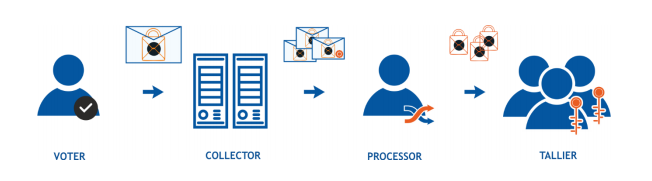
\includegraphics[width=\textwidth]{images/Główne częsci systemu estońskiego.png}

Główne częsci systemu:
\begin{itemize}
    \item Voter (dalej nazywany wyborcą) - za pośrednictwem aplikacji klienckiej (która w systemie estońskim jest aplikacją desktopową pobieraną przed wyborami) szyfruje i zatwierdza swoim podpisem elektronicznym głos, który następnie wysyłany jest do Kolektora.
    \item Collector (dalej nazywany Kolektorem) - to aplikacja serwerowa wyposażona w logikę pozwalającą na utworzenie głosu. Aplikacja waliduje dane wprowadzone przez wyborce i elektronicznie podpisuje dane, które następnie przesyła do Procesora.
    \item Processor (dalej nazywany Procesorem) - zajmuje się przetwarzaniem głosów. Sprawdza poprawność danych otrzymanych z Kolektora, wraz z podpisem elektronicznym. Usuwa głosy, które się powtarzają, zarówno głosy oddane elektronicznie, jak i te oddane w lokalach wyborczych. Sortuje głosy według okręgów wyborczych i usuwa z nich podpis elektroniczny, w celu anonimizacji głosu. Tak przetworzone głosy są mieszane według odpowiedniego algorytmu i wysyłane do Licznika.
    \item Tallier (dalej nazywany Licznikiem) - rolą licznika jest odebranie głosu od Procesora, otwarcie go i dodanie przyporządkowanie do odpowiedniego wyniku.
\end{itemize}
\chapter{Projekt systemu}
System został zaprojektowany od strony teoretycznej, co oznacza wyszczególnienie modułów systemu, aktorów, przypadków użycia, modelów baz danych i wykorzystanych technologii. Obecny rozdział zawiera przegląd opracowanego rozwiązania oraz jego teoretyczny opis.

\section{Diagram przypadków użycia.}

W systemie można wyróżnić dwóch aktorów: wyborcę i administratora wyborów. Wyborca posiada funkcje typowe dla użytkownika serwisu internetowego. Posiada swoje konto, które po zalogowaniu udostępnia mu jako główną funkcję systemu, czyli możliwość oddania głosu. W celu oddania głosu użytkownik musi wybrać odpowiednie głosowanie, które jest dostarczane za pomocą API. Użytkownik może być przypisany do kilku trwających, bądź zaplanowanych głosowań. Po wyborze głosowania wyborca musi wybrać, na którego kandydata będzie głosował. Po wybraniu odpowiedniej kandydatury, wyborca wysyła swój głos. Wysłanie głosu jest równoznaczne z zakończeniem procesu głosowania. Dla każdego głosowania wyborca może wysłać tylko jeden głos, na jednego kandydata. Po wysłaniu głosów, użytkownik może się wylogować. W przypadku problemów z przejściem przez proces wyborczy, użytkownik może przeczytać instrukcję obsługi, która zawiera informacje o kolejnych krokach procesu wyborczego. Dodatkowo użytkownik może przeglądać wyniki wyborów, w których brał udział.

\begin{figure}[h]
    \centering
    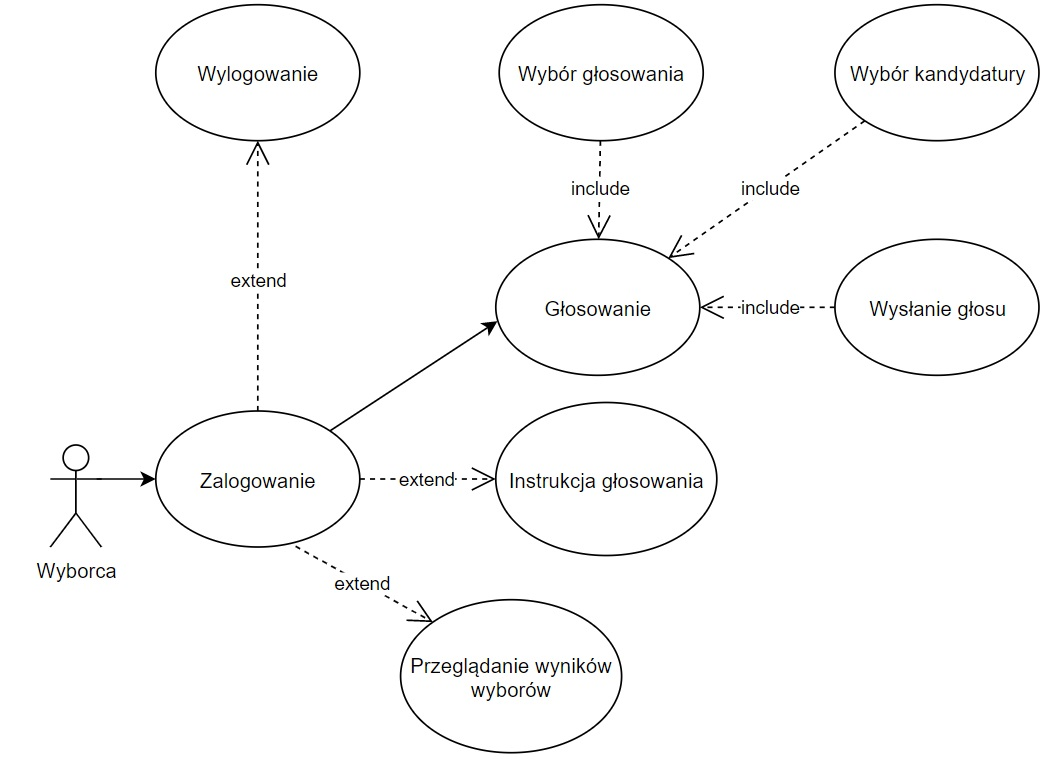
\includegraphics[scale=0.4]{images/user_use_case.jpg}
    \caption{Diagram przypadków użycia dla wyborcy.}
\end{figure}

\newpage

Administrator wyborów również posiada swoje konto, dzięki któremu musi się zalogować, aby mieć możliwość korzystania ze swoich funkcji. Głównym zadaniem administratora jest stworzenie wyborów. Tworzenie wyborów to proces odbywający się w kilu krokach. Pierwszym krokiem jest podanie odpowiedniego tytułu wyborów, opisu, daty rozpoczęcia i zakończenia oraz przypisania adresu serwera bazy danych, która przechowuje głosy. Etap ten jest określany jako konfiguracja wyborów. Następnym krokiem jest dodanie odpowiednich kandydatów oraz krótkich opisów. Ostatnim krokiem jest przypisanie wyborców dostępnych w bazie danych, dla których będą udostępnione wybory. Tak utworzone i skonfigurowane wybory, są dodawane do bazy danych.
Baza danych przechowująca konta wyborców może być w dowolnym momencie modyfikowana, poprzez stworzenie nowego konta wyborcy, bądź jego usunięcie. Administrator może również w niewielkim stopniu modyfikować trwające wybory, poprzez przypisanie nowego wyborcy i zmianę serwera bazy danych przechowującej głosy, w przypadku awarii. Jednym z najważniejszych zadań administratora jest ogłoszenie wyników wyborów. Po ogłoszeniu wyników wyborów, nie można dodawać głosów, a wyniki wyborów są udostępniane wyborcom.

\begin{figure}[h]
    \centering
    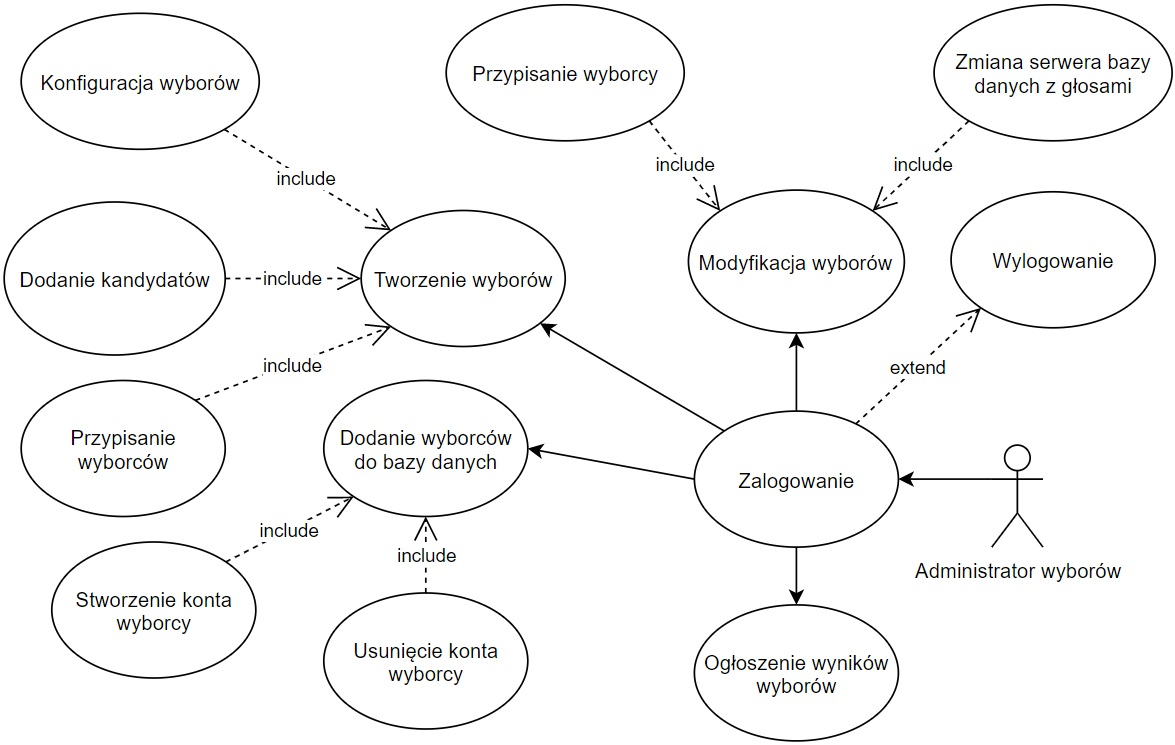
\includegraphics[scale=0.4]{images/admin_use_case.jpg}
    \caption{Diagram przypadków użycia dla administratora wyborów.}
\end{figure}

\section{Podział systemu na moduły.}
System można podzielić na 4 moduły, które wchodzące ze sobą w interakcje tworzą spójną i działającą aplikację. Do tych modułów należą:
\begin{itemize}
    \item Serwer udostępniający API oraz baza danych.
    \item Aplikacja webowa wyborcy.
    \item Aplikacja webowa administratora.
    \item Sieci Blockchain, przechowujące głosy, tworzone indywidualnie dla każdego głosowania.
\end{itemize}

\newpage

\begin{figure}[h]
    \centering
    \includegraphics[scale=0.4]{images/moduły_systemu.jpg}
    \caption{Schemat przedstawiający moduły systemu.}
\end{figure}

\newpage

\section{API i baza danych.}

\begin{figure}[h]
    \centering
    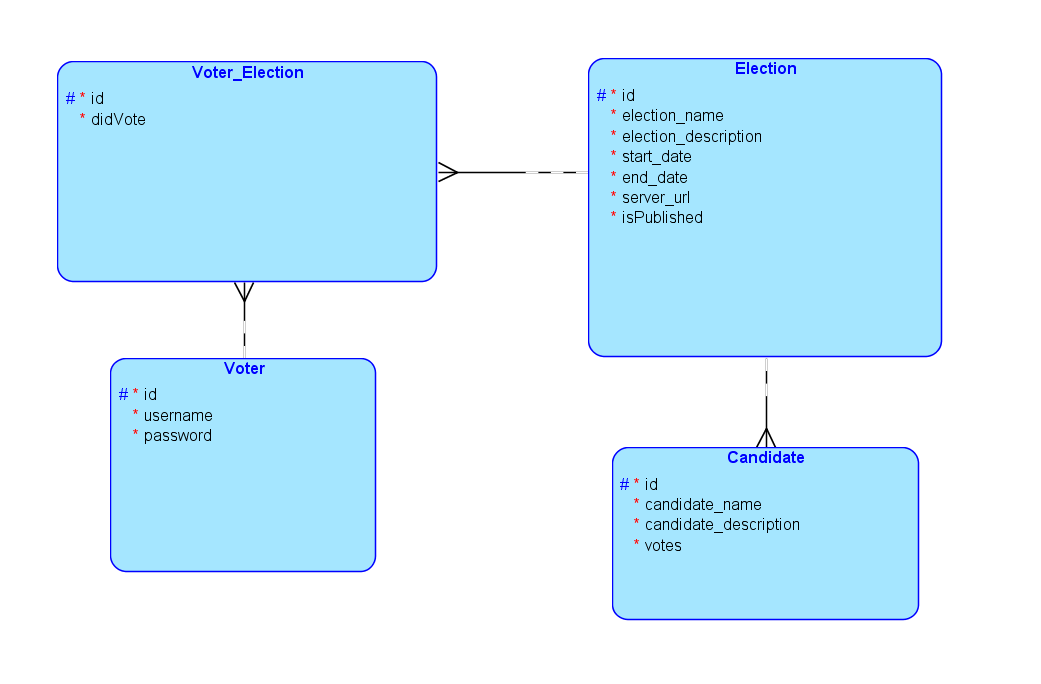
\includegraphics[scale=0.4]{images/Logical.png}
    \caption{Model logiczny bazy danych.}
\end{figure}

\begin{figure}[h]
    \centering
    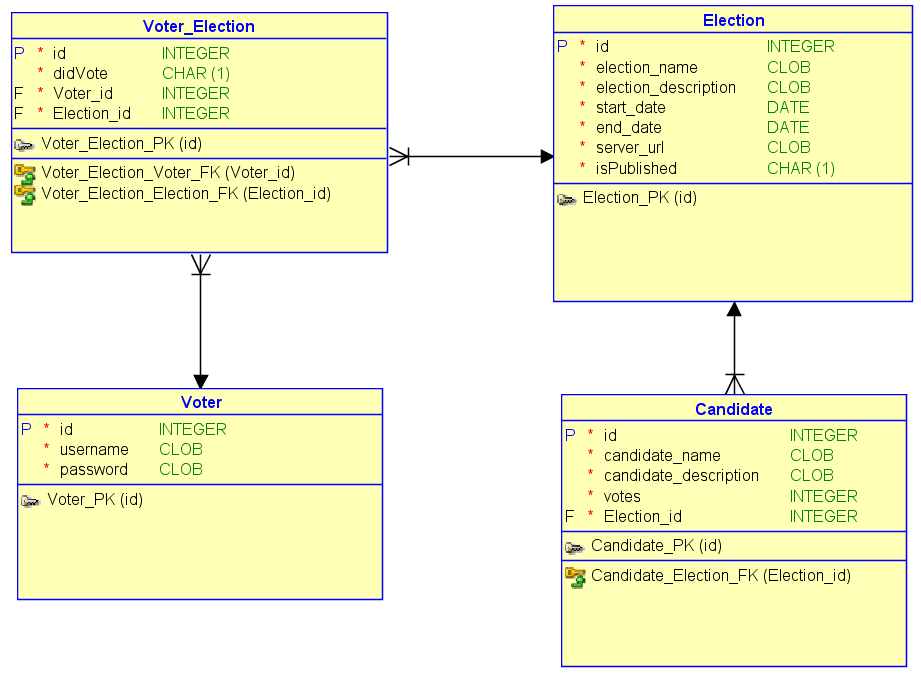
\includegraphics[scale=0.4]{images/Relational.png}
    \caption{Model fizyczny bazy danych}
\end{figure}

\end{document}
